\chapter{Analisis}
\label{chap:analisis}

Pada bab ini akan dijelaskan mengenai analisis grafik dari data sensor-sensor pada \textit{smartphone} ketika sedang mengangguk dan menggeleng, analisis aplikasi-aplikasi sejenis, dan analisis metode pendeteksi gerakan kepala. 

\section{Analisis Grafik Data Sensor-sensor pada \textit{Smartphone} Android }
\label{sec:analisis_grafik_data}

Pada analisis ini akan dilakukan perekaman mengganguk dan menggeleng dengan sensor-sensor pada Android. Perekaman-perekaman ini akan dilakukan pada tiga kondisi muka pengguna. Kondisi muka yang pertama adalah kondisi muka pengguna ketika menghadap ke depan. Kondisi muka yang kedua adalah kondisi muka pengguna keita menghadap ke atas sekitar $45^{\circ}$ dari pandangan muka menghadap ke atas. Kondisi muka yang ketiga adalah kondisi muka ketika menghadap serong ke kiri atas. Anggukan yang dilakukan oleh pengguna hanya sebanyak satu kalu mengangguk ke bawah saja. Sedangkan dalam menggeleng akan bergerak ke kiri terlebih dahulu dan ke kanan setelahnya dan diakhiri pada posisi muka kembali ke posisi awal.

Grafik-grafik yang akan ditunjukkan pada bab ini akan memiliki beberapa karakteristik. Sumbu y pada grafik yang akan ditunjukkan akan merepresentasikan besar nilainya, Sedangkan sumbu x akan merepresentasikan waktunya. Grafik yang ditunjukkan akan memiliki beberapa nilai, tergantung dari jumlah nilai yang dikembalikan untuk setiap sensornya. Contohnya pada sensor \textit{accelerometer} yang memiliki tiga jenis nilai, sehingga pada grafik akan terbentuk tiga buah garis nilai. Aplikasi akan merekam beberapa sensor secara langsung ketika pengguna mengangguk atau menggeleng, sehingga nilai wakunya akan sama untuk kondisi muka yang sama walaupun sensornya berbeda.

Analisis grafik data sensor-sensor pada Android dilakukan dengan membuat suatu aplikasi perekam sensor-sensor yang ada pada \textit{smartphone} Android terlebih dahulu. Aplikasi ini akan merekam nilai-nilai yang dihasilkan dari sebagian sensor-sensor pada android setiap ada perubahan. Pada skripsi ini, nilai sensor-sensor yang dibutuhkan adalah sensor \textit{accelerometer}, \textit{gyroscope}, \textit{rotation vector}, dan \textit{geomagnetic rotation}. Aplikasi menyimpan nilai sensor-sensor menggunakan format CSV \textit{(Comma Separated Values)}. Dari data yang diperoleh oleh apliasi tersebut dibuatkan grafiknya menggunakan aplikasi Microsoft Excel. Penjelasan dari setiap grafik akan dijelaskan pada subbab-subbab berikut.
\subsection{Analisis Grafik Sensor \textit{Accelerometer}}
\label{sec:analisis_grafik_sensor_accelerometer}
Seperti yang sudah dijelaskan pada bab sebelumnya, sensor \textit{accelerometer} akan mendeteksi seluruh percepatan yang terjadi pada perangkat Android. Perekaman ini perangkat android akan diletakkan di depan muka pengguna, sehingga percepatan yang mempengaruhi perangkat Android hanya percepatan gravitasi dengan percepatan yang dilakukan oleh gerakan kepala pengguna. Gambar \ref{fig:grafik-sensor-accelerometer-mengangguk-depan} merupakan grafik yang terbentuk dari nilai yang di terima oleh sensor \textit{accelerometer} ketika pengguna mengangguk dan sedang menghadap ke depan.

\begin{figure}[htbp]
\centering
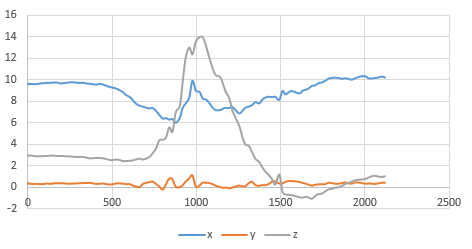
\includegraphics[scale=1]{Gambar/grafik-sensor-accelerometer-mengangguk-depan.png}
\caption{Gambar grafik nilai sensor \textit{accelerometer} ketika pengguna mengangguk dan sedang menghadap ke depan.} 
\label{fig:grafik-sensor-accelerometer-mengangguk-depan}
\end{figure}
Pada Gambar \ref{fig:grafik-sensor-accelerometer-mengangguk-depan} terlihat nilai z menaik dan nilai x menurun ketika sedang mengangguk. Tetapi nilai x kembali menaik ketika nilai z sudah hampir mencapai nilai tertinggi. Sedangkan nilai y terlihat cukup konstan di sekitar angka 0. Kemudian Gambar \ref{fig:grafik-sensor-accelerometer-mengangguk-atas} merupakan grafik yang terbentuk dari nilai yang diterima oleh sensor \textit{accelerometer} ketika pengguna mengangguk dan sedang menghadap ke atas.

\begin{figure}[htbp]
\centering
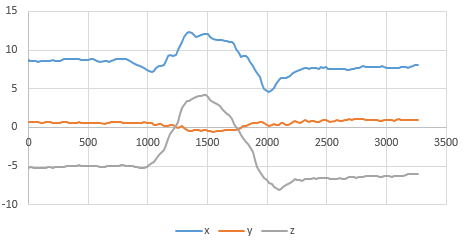
\includegraphics[scale=1]{Gambar/grafik-sensor-accelerometer-mengangguk-atas.png}
\caption{Gambar grafik nilai sensor \textit{accelerometer} ketika pengguna mengangguk dan sedang menghadap ke atas.} 
\label{fig:grafik-sensor-accelerometer-mengangguk-atas}
\end{figure}

Pada Gambar \ref{fig:grafik-sensor-accelerometer-mengangguk-atas} terlihat nilai x dengan y memiliki pola yang serupa ketika mengangguk. Kedua nilai menaik ketika pengguna sedang mengangguk. Nilai x bermulai dari nilai sekitar sebesar 9 sedangkan nilai z bernilai sekitar sebesar -5. Sama seperti pada Gambar \ref{fig:grafik-sensor-accelerometer-mengangguk-depan} nilai y terlihat konstan di sekitar angka 0. Selanjutnya Gambar \ref{fig:grafik-sensor-accelerometer-mengangguk-kiri-atas} merupakan grafik yang terbentuk dari nilai yang diterima oleh sensor \textit{accelerometer} ketika pengguna mengangguk dan sedang menghadap ke kiri atas.


\begin{figure}[htbp]
\centering
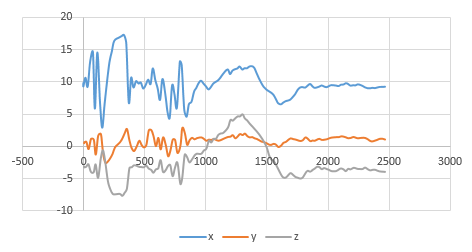
\includegraphics[scale=1]{Gambar/grafik-sensor-accelerometer-mengangguk-kiri-atas.png}
\caption{Gambar grafik nilai sensor \textit{accelerometer} ketika pengguna mengangguk dan sedang menghadap ke kiri atas.} 
\label{fig:grafik-sensor-accelerometer-mengangguk-kiri-atas}
\end{figure}

Pada Gambar \ref{fig:grafik-sensor-accelerometer-mengangguk-kiri-atas} grafik tersebut terlihat berantakan. Pada Grafik ini sulit untuk membedakan kondisi kapan pengguna sedang mengangguk. Goncangan yang terjadi terhadap \textit{smartphone}, seperti munculnya notifikasi mungkin dapat menyebabkan hal ini. Namun pada waktu mencapai 1000 milidetik terlihat cukup stabil. Pada Gambar \ref{fig:grafik-sensor-accelerometer-mengangguk-kiri-atas} juga menunjukkan bahwa nilai x dengan z memiliki pola yang sama hingga akhir, dan nilai y konstan di sekitar angka 0. Hasil nilai tersebut serupa dengan kasus ketika menghadap ke atas. Gambar \ref{fig:grafik-sensor-accelerometer-menggeleng-depan} merupakan grafik yang terbentuk dari nilai yang diterima oleh sensor \textit{accelerometer} ketika pengguna menggeleng dan sedang menghadap ke depan.

\begin{figure}[htbp]
\centering
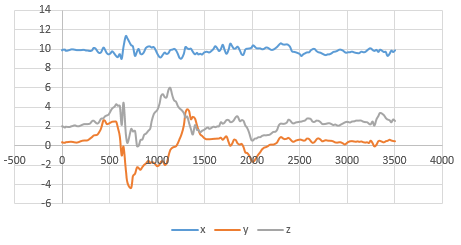
\includegraphics[scale=1]{Gambar/grafik-sensor-accelerometer-menggeleng-depan.png}
\caption{Gambar grafik nilai sensor \textit{accelerometer} ketika pengguna menggeleng dan sedang menghadap ke depan.} 
\label{fig:grafik-sensor-accelerometer-menggeleng-depan}
\end{figure}

Pada grafik di Gambar \ref{fig:grafik-sensor-accelerometer-menggeleng-depan}, nilai x konstan di sekitar angka 10. Nilai y dengan z menaik dan menurun ketika pengguna menggelengkan kepala. Berbeda dengan kasus pada Gambar \ref{fig:grafik-sensor-accelerometer-mengangguk-atas} dan pada Gambar \ref{fig:grafik-sensor-accelerometer-mengangguk-kiri-atas} yang nilai x dengan z memiliki pola yang serupa, sedang pada kasus ini nilai y dan z tidak memiliki pola yang serupa. Kemudian pada Gambar \ref{fig:grafik-sensor-accelerometer-menggeleng-atas} menunjukan grafik yang terbentuk dari nilai yang diterima oleh sensor \textit{accelerometer} ketika pengguna menggeleng dan sedang menghadap ke atas.

\begin{figure}[htbp]
\centering
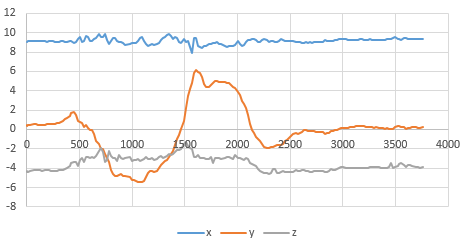
\includegraphics[scale=1]{Gambar/grafik-sensor-accelerometer-menggeleng-atas.png}
\caption{Gambar grafik nilai sensor \textit{accelerometer} ketika pengguna menggeleng dan sedang menghadap ke atas.} 
\label{fig:grafik-sensor-accelerometer-menggeleng-atas}
\end{figure}

Berbeda dengan kasus pada Gambar \ref{fig:grafik-sensor-accelerometer-menggeleng-depan}, nilai x pada grafik di Gambar \ref{fig:grafik-sensor-accelerometer-menggeleng-atas} terlihat konstan di sekitar nilai 10 dan nilai z di sekitar nilai -3. Nilai y mengalami kenaikan dan penurunan saat menggeleng. Gambar \ref{fig:grafik-sensor-accelerometer-menggeleng-atas} menunjukan grafik yang terbentuk dari nilai yang diterima oleh sensor \textit{accelerometer} ketika pengguna menggeleng dan sedang menghadap ke kiri atas.

\begin{figure}[htbp]
\centering
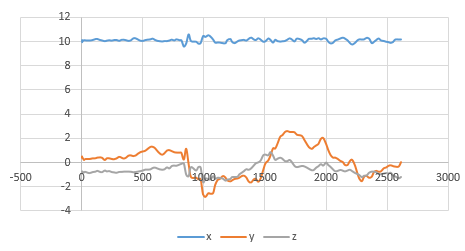
\includegraphics[scale=1]{Gambar/grafik-sensor-accelerometer-menggeleng-kiri-atas.png}
\caption{Gambar grafik nilai sensor \textit{accelerometer} ketika pengguna menggeleng dan sedang menghadap ke kiri atas.} 
\label{fig:grafik-sensor-accelerometer-menggeleng-kiri-atas}
\end{figure}

Pada grafik di Gambar \ref{fig:grafik-sensor-accelerometer-menggeleng-kiri-atas} nilai x konstan di sekitar nilai 10. Nilai y menaik dan menurun, tetapi tidak beraturan. Nilai pada z juga mengalami sedikit kenaikan dan penurunan. 

Dari keenam grafik tersebut terlihat bahwa nilai yang terpengaruh ketika pengguna sedang mengangguk adalah nilai x dengan z. Nilai y tidak berpengaruh karena nilai y cenderung konstan. Nilai yang terpengaruh ketika pengguna sedang menggeleng adalah nilai y. Nilai x terlihat konstan pada setiap grafik, tetapi nilai z mengalami sedikit pergerakan ketika pengguna sedang mengangguk sehingga tidak dapat dipastikan bahwa nilai z terpengaruhi gerakan menggeleng. 

\subsection{Analisis Grafik Sensor \textit{Gyroscope}}
\label{sec:analisis_grafik_sensor_gyroscope}
Perekaman menggunakan sensor \textit{gyroscope} akan mendapatkan percepatan angular yang terjadi setiap waktunya. Berbeda dengan sensor \textit{accelerometer} yang dapat terpengaruhi oleh lingkungan sekitar seperti gravitasi dan percepatan lainnya, sensor ini hanya akan merekam perputaran yang terjadi pada perangkat saja. Hal ini sangat menguntungkan dalam mendeteksi suatu gerakan karena tidak harus memperdulikan kasus dari pengaruh luar. Gambar \ref{fig:grafik-sensor-gyroscope-mengangguk-depan} menunjukkan nilai-nilai sensor \textit{gyroscope} ketika pengguna sedang mengangguk dan menghadap ke depan.


\begin{figure}[htbp]
\centering
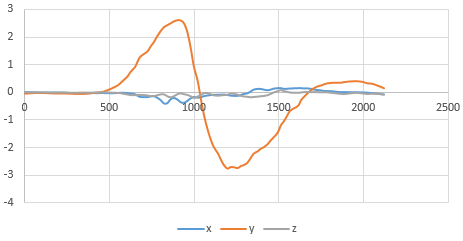
\includegraphics[scale=1]{Gambar/grafik-sensor-gyroscope-mengangguk-depan.png}
\caption{Gambar grafik nilai sensor \textit{gyroscope} ketika pengguna mengangguk dan sedang menghadap ke depan.} 
\label{fig:grafik-sensor-gyroscope-mengangguk-depan}
\end{figure}

Grafik pada Gambar \ref{fig:grafik-sensor-gyroscope-mengangguk-depan} terbentuk 1 buah bukit dan lembah pada nilai y. Bukit yang terjadi disini menunjukkan ketika pengguna menggerakan kepalanya kebawah, dan ketika kepala pengguna kembali ke posisi semula percepatan angularnya berbalik arah sehingga menimbulkan lembah. Nilai x dengan z cenderung bernilai 0. Gambar \ref{fig:grafik-sensor-gyroscope-mengangguk-atas} menunjukkan nilai-nilai sensor \textit{gyroscope} ketika pengguna sedang mengangguk dan menghadap ke atas.

\begin{figure}[htbp]
\centering
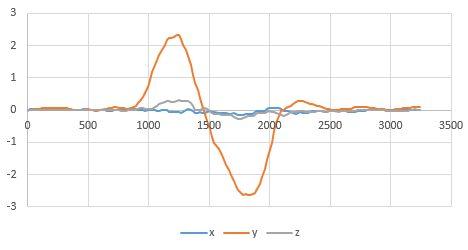
\includegraphics[scale=1]{Gambar/grafik-sensor-gyroscope-mengangguk-atas.png}
\caption{Gambar grafik nilai sensor \textit{gyroscope} ketika pengguna mengangguk dan sedang menghadap ke atas.} 
\label{fig:grafik-sensor-gyroscope-mengangguk-atas}
\end{figure}

Grafik pada Gambar \ref{fig:grafik-sensor-gyroscope-mengangguk-depan} mirip seperti grafik pada Gambar \ref{fig:grafik-sensor-gyroscope-mengangguk-atas}. Begitu pula pada grafik di Gambar \ref{fig:grafik-sensor-gyroscope-mengangguk-kiri-atas} yang memiliki pola yang serupa dengan yang grafik-grafik sebelumnya.

\begin{figure}[htbp]
\centering
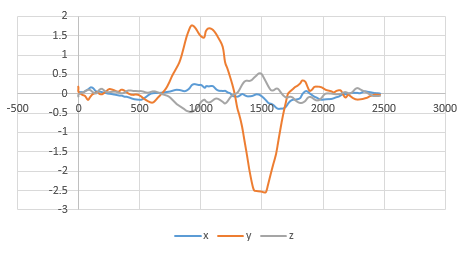
\includegraphics[scale=1]{Gambar/grafik-sensor-gyroscope-mengangguk-kiri-atas.png}
\caption{Gambar grafik nilai sensor \textit{gyroscope} ketika pengguna mengangguk dan sedang menghadap ke kiri atas.} 
\label{fig:grafik-sensor-gyroscope-mengangguk-kiri-atas}
\end{figure}

Pada grafik di Gambar \ref{fig:grafik-sensor-gyroscope-menggeleng-depan} nilai yang mengalami kenaikan dan penurunan adalah nilai x dan nilai-nilai lainnya cenderung berada pada nilai 0. Nilai x membentuk 2 buah bukit dan 1 buah lembah. Bukit pertama terjadi ketika pengguna menggerakan kepalanya ke kiri. Lembah pertama terjadi ketika pengguna menggerakan kepalanya ke kanan. Bukit kedua terjadi ketika pengguna menggerakan kepalanya kembali ke posisi semula.

\begin{figure}[htbp]
\centering
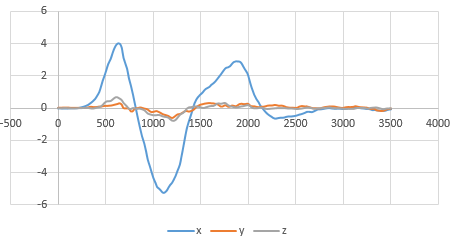
\includegraphics[scale=1]{Gambar/grafik-sensor-gyroscope-menggeleng-depan.png}
\caption{Gambar grafik nilai sensor \textit{gyroscope} ketika pengguna menggeleng dan sedang menghadap ke depan.} 
\label{fig:grafik-sensor-gyroscope-menggeleng-depan}
\end{figure}

Pada grafik di Gambar \ref{fig:grafik-sensor-gyroscope-menggeleng-atas} dengan grafik di Gambar \ref{fig:grafik-sensor-gyroscope-menggeleng-kiri-atas} menunjukkan pola grafik yang serupa dengan grafik pada Gambar \ref{fig:grafik-sensor-gyroscope-menggeleng-depan}.

\begin{figure}[htbp]
\centering
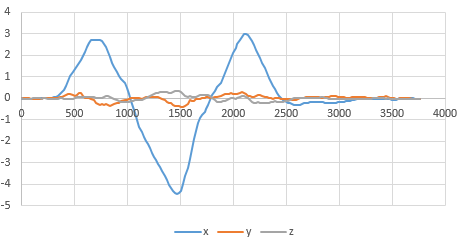
\includegraphics[scale=1]{Gambar/grafik-sensor-gyroscope-menggeleng-atas.png}
\caption{Gambar grafik nilai sensor \textit{gyroscope} ketika pengguna menggeleng dan sedang menghadap ke atas.} 
\label{fig:grafik-sensor-gyroscope-menggeleng-atas}
\end{figure}

\begin{figure}[htbp]
\centering
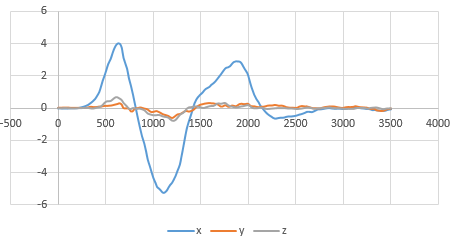
\includegraphics[scale=1]{Gambar/grafik-sensor-gyroscope-menggeleng-depan.png}
\caption{Gambar grafik nilai sensor \textit{gyroscope} ketika pengguna menggeleng dan sedang menghadap ke kiri atas.} 
\label{fig:grafik-sensor-gyroscope-menggeleng-kiri-atas}
\end{figure}

Dari hasil-hasil tersebut dapat disimpulkan bahwa arah pandang pengguna tidak mempengaruhi sensor \textit{gyroscope} dalam mendeteksi gerakan kepala. Nilai-nilai yang dikembalikan oleh sensor \textit{gyroscope} memiliki  pola grafik yang jauh lebih rapih dibandingkan grafik-grafik yang dihasilkan oleh sensor \textit{accelerometer}. Selain itu sensor gyroscope hanya menggunakan 1 jenis nilai yang dipengaruhi oleh pergerakan kepala, sedangkan accelerometer ada 2 jenis nilai yang di pengaruhi gerakan kepala pada saat mengangguk. Oleh karena itu sensor gryoscope lebih baik dalam mendeteksi gerakan yang terjadi pada perangkat android.

\subsection{Analisis Grafik Sensor \textit{Rotation Vector}}
\label{sec:analisis_grafik_sensor_rotation_vector}

